\documentclass[11pt,a4paper,UTF8,fontset=windows]{ctexart}
\usepackage[margin=25mm]{geometry}
\usepackage{amsmath,amssymb,booktabs,graphicx,fancyhdr,hyperref,float}
\hypersetup{colorlinks=true,linkcolor=blue,urlcolor=blue,citecolor=blue}
\pagestyle{fancy}\fancyhf{}\fancyhead[C]{队伍：TEAM NUMBER REQUIRED}\fancyfoot[C]{\thepage}
\setlength{\headheight}{15pt}\setlength{\parskip}{3pt}\setlength{\parindent}{0pt}
\usepackage{caption}
\captionsetup{font=small,labelfont=bf}
\graphicspath{{../../img/中文/}}
\begin{document}
\begin{center}
{\large 队伍：TEAM NUMBER REQUIRED}\par\vspace{12mm}
{\Large B 题}\par\vspace{10mm}
{\LARGE 由 0.10 秒运动预测点球}\par\vspace{8mm}
\end{center}
\vspace{6mm}
\begin{center}
{\small 中文译本仅供队友阅读，队号待定，正式提交以英文稿为准。}
\end{center}
\vspace{4mm}
\begin{abstract}
题给点球早期的两个位置，但风、空气密度和阻力系数都没有测量。本文只用一个明确的受力模型，回答球的其余飞行可能是什么样。模型从出脚到球门平面全程考虑重力、相对空气的二次阻力和写成叉乘的有效侧向力；侧向项不是自旋的测量，而是自旋与升力的合并效果。对每一组列出的风速、密度和阻力系数，我们用两个位置反求初速度与两个侧向系数。只有六个坐标残差都在允许误差内，这组参数才被接受。列出的一共有 210 组参数，其中 86 组在 5 mm 允许误差下被接受；它们的球门平面坐标覆盖 $y\in[2.5384,2.6812]$ m、$z\in[1.9451,1.9867]$ m，两条被接受的轨迹落点相距 0.1477 m。当前示例取风速 8.0 m/s、密度 1.225 kg/m$^3$、$C_D=0.350$，球心在 0.4042 s 时穿过球门平面于 $(2.6087,1.9598)$ m。落点的分散说明两次观测不能选出唯一落点，但它不是概率。MATLAB 检查包括三档步长、功与能平衡和事件检查。没有独立的实测全程飞行，因此这些检查验证计算过程，模型还需实测飞行确认。只搜索列出的参数，图中的范围不能保证包含所有可能情况。
\end{abstract}
\clearpage

\section{问题与求解思路}
本节说明我们计算什么，以及全文按什么顺序阅读。

球心在出脚时的位置为 $\mathbf r_0=(0,0,0.11)$ m，另外两个时刻为 $t_1=0.05$ s 与 $t_2=0.10$ s：
\begin{equation}
\mathbf r_1=(1.50, 0.45, 0.44)\ \mathrm m,\qquad
\mathbf r_2=(2.96, 0.86, 0.74)\ \mathrm m.
\end{equation}
取 $x$ 指向球门、$y$ 平行球门线、$z$ 向上。这六个数就是全部位置数据。风、密度、阻力和出脚条件都未知，因而一条轨迹并不能被唯一确定。我们改问：对一组列出的环境取值，哪些出脚条件能在允许误差内重现两个位置，这些轨迹又在哪里穿过 $x=11$ m？阅读顺序如下：第 2 节写出受力方程，第 3 节说明观测如何筛出参数取值，第 4 节给出数字和插图，第 5 节列出计算检查与适用范围，第 6 节回答问题。

本文保留同时满足允许误差和物理检查的轨迹。图~\ref{fig:flow}展示计算顺序：先设定环境，再求出脚条件，最后检查整段飞行。未通过检查的结果也会记录。
\begin{figure}[H]\centering
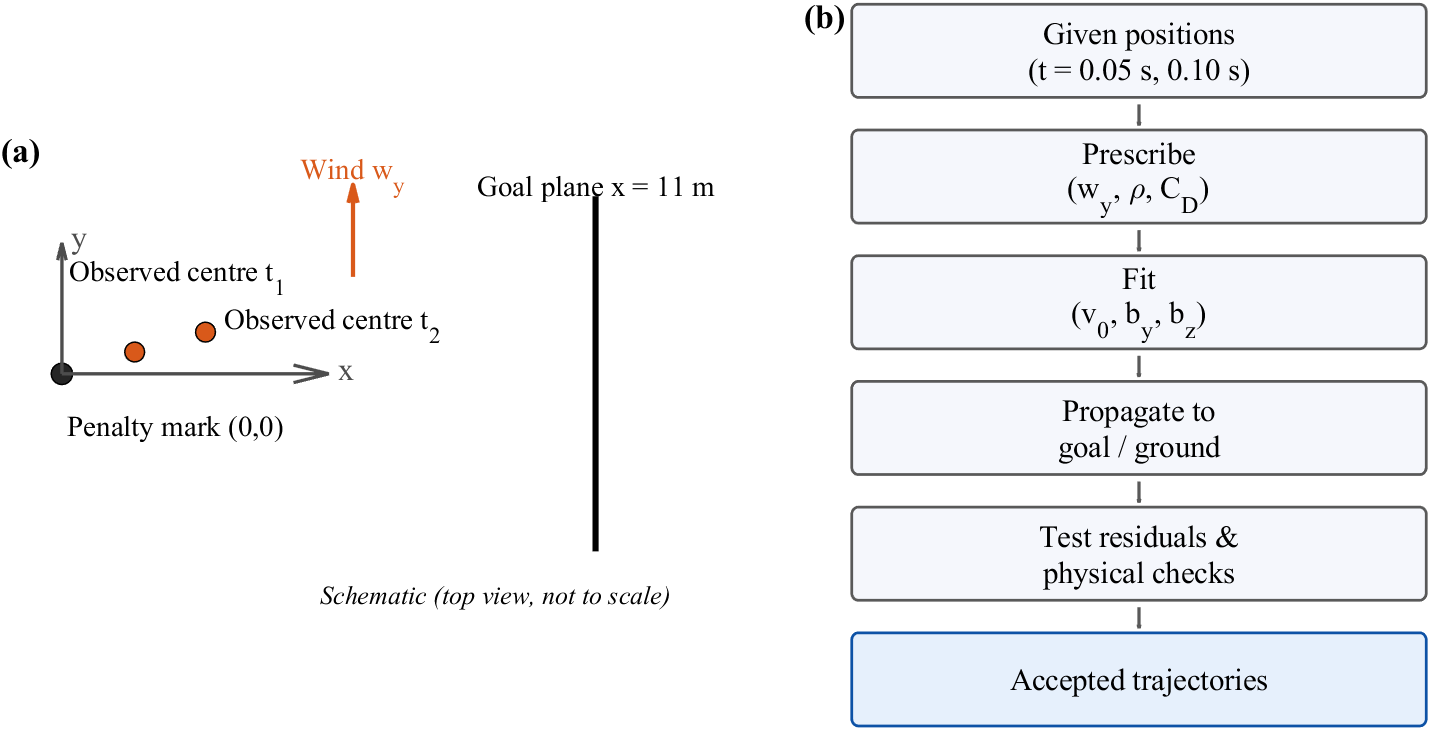
\includegraphics[width=\linewidth]{系统与反演流程.png}
\caption{坐标约定与从两次观测到符合观测轨迹的流程。左图为水平几何示意；右图给出列出的环境取值、反求出的出脚条件、允许误差与物理检查，以及记录下来的终止事件。}
\label{fig:flow}
\end{figure}

\section{从出脚到球门的物理模型}

本节依次回答三个问题：球受到什么力，这些力怎样写成方程，哪些简化会影响最后的预测。先建立受力依据，再使用方程计算。
\subsection{研究对象、坐标和初始条件}
研究对象是已经离脚、尚未碰到地面或门柱的足球。取球心位置$\mathbf r=(x,y,z)$，速度$\mathbf v=\dot{\mathbf r}$，$x$轴指向球门，$z$轴向上。球半径$R=0.11$ m、质量$m=0.43$ kg；初始球心按题目固定，初速度待求：
\begin{equation}
\mathbf r(0)=(0,0,R),\qquad \mathbf v(0)=\mathbf v_0,\qquad
\mathbf g=(0,0,-9.81)\ \mathrm{m\,s^{-2}}.
\end{equation}
质量和周长$2\pi R$符合IFAB球规格~\cite{ifab}，但不表示测得了本题足球的质量与材料。脚的作用已通过$\mathbf v_0$体现；球离脚后不再承受脚的推力。忽略形变后的球心平动满足牛顿第二定律：
\begin{equation}
m\dot{\mathbf v}=\mathbf F_g+\mathbf F_D+\mathbf F_M,\qquad \mathbf F_g=m\mathbf g.
\label{eq:newton}
\end{equation}
接下来分别建立阻力$\mathbf F_D$和侧向力$\mathbf F_M$，而不是直接从位置曲线猜加速度。
\subsection{从相对气流得到阻力}
空气动力取决于球相对空气的速度。设本次射门期间横风近似不变，$\mathbf w=(0,w_y,0)$，定义
\begin{equation}
\mathbf u=\mathbf v-\mathbf w,\quad U=\|\mathbf u\|,\quad
A=\pi R^2,\quad p_{\rm dyn}=\tfrac12\rho U^2.
\end{equation}
$p_{\rm dyn}$是动压，乘迎风面积得到力的尺度。把球面接缝、边界层和分离等影响收进无量纲阻力系数$C_D$，便有~\cite{nasa}
\begin{equation}
D=p_{\rm dyn}AC_D,\qquad
\mathbf F_D=-D\frac{\mathbf u}{U}
=-\tfrac12\rho AC_DU\mathbf u.
\label{eq:drag}
\end{equation}
负号规定阻力与相对气流反向；$\rho AU^2$的单位是N。式中并非既有“运动阻力”又额外加一份“风阻”：风通过$\mathbf u$改变同一项空气动力。动压给出量级，$C_D$仍需实验标定，不能只用伯努利方程或能量守恒把它推定为某个数。
\subsection{为什么使用有效侧向力}
旋转会改变球两侧的边界层与尾流，使气动力出现垂直于气流的分量。足球风洞实验支持这一机制，也显示系数与旋转、流态有关~\cite{asai}。用通常的力系数定义，侧向力大小为
\begin{equation}
F_M=\tfrac12\rho AU^2C_L.
\end{equation}
为了连接到可计算的向量形式，记$\boldsymbol\omega_\perp$为角速度垂直于$\mathbf u$的部分。若在有限速度范围内近似$C_L\simeq c_sR\|\boldsymbol\omega_\perp\|/U$，其中$c_s$为无量纲系数，并取方向沿$\boldsymbol\omega\times\mathbf u$，则
\begin{equation}
\mathbf F_M\simeq\tfrac12\rho Ac_sR(\boldsymbol\omega\times\mathbf u)
=m(\mathbf b\times\mathbf u),\qquad
\mathbf b=\frac{\rho Ac_sR}{2m}\boldsymbol\omega.
\label{eq:magnus}
\end{equation}
这一步是局部经验近似，不是风洞文献证明的普适线性定律。$\mathbf b$的单位是s$^{-1}$，把真实自旋与未知的气动效率$c_s$合在一起。两帧位置无法分别确定它们，因此程序只求有效$\mathbf b$，不把它解释成实测角速度。

本文取$\mathbf b=(0,b_y,b_z)$，使主要沿$x$方向运动的球，其横向和竖向偏转分别由$b_z$和$b_y$描述。令$b_x=0$是减少未知量的假设，并不说明真实球的这个分量必为零。若要预测自旋本身，还需转动惯量和空气力矩去求$\mathbf I\dot{\boldsymbol\omega}=\boldsymbol\tau$；题目没有这些数据。保持$\mathbf b$恒定只代表在约0.4s内使用恒定有效参数，其误差须留在模型局限中。
\subsection{合成完整运动方程}
将式~\eqref{eq:drag}、\eqref{eq:magnus}代入牛顿方程，并令$K=\rho A/(2m)$，得到程序实际积分的六个一阶方程：
\begin{align}
\dot{\mathbf r}&=\mathbf v,\qquad
\dot{\mathbf v}=\mathbf g-KC_DU\mathbf u+\mathbf b\times\mathbf u,\label{eq:model}\\
\dot v_x&=-KC_DUv_x+b_yv_z-b_z(v_y-w_y),\nonumber\\
\dot v_y&=-KC_DU(v_y-w_y)+b_zv_x,\nonumber\\
\dot v_z&=-g-KC_DUv_z-b_yv_x,\qquad g=\|\mathbf g\|.\nonumber
\end{align}
分量式也说明三种运动相互影响：横风不仅改变$y$方向阻力，$v_y-w_y$还进入$x$方向侧力。改变某一参数后，必须重新计算整个向量状态。
\begin{table}[H]\centering\small
\caption{本节符号及其角色。}\begin{tabular}{lll}\toprule
符号 & 含义 & 单位或来源\\\midrule
$\mathbf r,\mathbf v,\mathbf u$ & 位置、地面速度、相对空气速度 & m；m/s；m/s\\
$m,R,A$ & 质量、半径、迎风面积 & kg；m；m$^2$\\
$\rho,w_y,C_D$ & 密度、横风、阻力系数 & 指定情景，不是实测\\
$\mathbf v_0,b_y,b_z$ & 初速度和有效侧力参数 & m/s；s$^{-1}$，待求\\
$K,C_L,C_\perp$ & 气动尺度、升力与侧力系数 & m$^{-1}$；无量纲\\
\bottomrule\end{tabular}\end{table}
\subsection{用量级判断哪些作用重要}
为判断是否能忽略某项，取当前示例出脚相对气流速度$U_0=31.26$ m/s、飞行时间$T=0.4042$ s。初始重力、阻力、侧力大小分别约为$4.22$、$7.96$、$6.96$ N，气动力与重力是同一量级。进一步比较它们在飞行时间内改变速度的相对大小：
\begin{equation}
\Pi_D=KC_DU_0T=0.239,\quad
\Pi_M=\|\mathbf b\|T=0.215,\quad
\Pi_g=\frac{gT}{U_0}=0.127.
\end{equation}
这些量均不远小于1，因此三项都保留。采用示例空气黏度$\mu=1.81\times10^{-5}$ Pa s和声速$c=343$ m/s，可估计
\begin{equation}
\mathrm{Re}=\frac{2\rho RU_0}{\mu}\simeq4.65\times 10^{5},\qquad
\mathrm{Ma}=\frac{U_0}{c}\simeq0.091.
\end{equation}
声速和黏度为量级估算所用的假设，不是场地测量。较小的马赫数支持忽略压缩性；雷诺数说明阻力系数与流态有关，所以恒定$C_D$是有限工况下的简化，不能因此认定它已被标定。

其余简化也要估计影响。空气浮力与重力之比约为$\rho(4\pi R^3/3)/m=1.59\%$；在不重新拟合出脚条件的估算中，忽略它可产生约$1.27$ cm的竖向位移差。因此本文不能把毫米级的计算残差说成毫米级的真实准确度。取地球自转角速度$\Omega=7.292115\times10^{-5}$ s$^{-1}$，其导致的位移量级$\Omega\|\mathbf v_0\|T^2$约为$0.39$ mm，低于本例允许误差。浮力、非恒定风和变化的气动系数仍会贡献模型误差，更多早期观测才能帮助检验它们。
\subsection{有风时怎样检查功与能}
令$E=\tfrac12m\|\mathbf v\|^2+mgz$。将牛顿方程与地面系速度点乘，重力势能项抵消后得到
\begin{align}
\frac{dE}{dt}&=(\mathbf F_D+\mathbf F_M)\cdot\mathbf v\label{eq:energy}\\
&=-\tfrac12\rho AC_DU^3+(\mathbf F_D+\mathbf F_M)\cdot\mathbf w.\nonumber
\end{align}
推导中用到了$\mathbf F_M\cdot\mathbf u=0$，但$\mathbf v=\mathbf u+\mathbf w$。所以侧向力对相对气流的瞬时功率为零，有风时对地面系的球仍可做功；不能强求球的地面系机械能一直下降。后面的功与能检查正是积分式~\eqref{eq:energy}，用于检验程序是否把力的方向和符号算对。


\section{用观测求参数}
本节说明两次位置如何变成一组组参数取值。

对每一组列出的 $\eta=(w_y,\rho,C_D)$，用有界非线性最小二乘反求 $q=(v_{0x},v_{0y},v_{0z},b_y,b_z)$：
\begin{equation}
q^*(\eta)=\arg\min_{q\in\mathcal B}\sum_{i=1}^{2}
\|\mathbf r(t_i;q,\eta)-\mathbf r_i\|^2,
\label{eq:fit}
\end{equation}
使用 \texttt{lsqnonlin}~\cite{lsq}，并从两个初值出发。拟合时用四阶Runge--Kutta方法，步长为$0.0025$ s；接受前另用\texttt{ode45}回代观测，RelTol=$10^{-11}$、AbsTol=$10^{-12}$。全程预测用RelTol=$10^{-9}$、AbsTol=$10^{-11}$、最大步长$0.002$ s。随后逐个检查六个坐标：
\begin{equation}
|r_j(t_i;q,\eta)-r_{ij}|\le\epsilon,
\qquad i=1,2,\quad j=x,y,z,
\label{eq:tol}
\end{equation}
分别在 $\epsilon=2,5,10,20$ mm 下筛选，默认取 5 mm。允许误差是明确声明的情景，不是测量得到的相机精度。

搜索使用 $[-8.000,8.000]$ m/s 上的 7 个风速、$\{1.100, 1.225, 1.350\}$ kg/m$^3$ 的 3 个密度值、以及 $[0.15,0.60]$ 上的 10 个阻力系数，共 210 组参数。这些是示例设置，不是实测分布。

一组参数还要通过物理筛选才算被接受：出脚方向向前且不向下，初速度在 10 到 40 m/s 之间，沿采样轨迹的侧力系数满足 $C_\perp\le0.50$；球在终止事件前必须位于地面以上，终止事件要在 2 s 内定位到。观测拟合与物理筛选分别记录，只有两项都通过才被接受。速度范围和 0.50 上限是保守的模型筛选，不是运动员或足球的普适极限。我们不强迫球进门：射偏也是记录下来的结果，球门只用来描述球飞到哪里。

结果之所以是一组轨迹而不是一次射门，有两个原因。第一，未知量比六个坐标多。改变风速或阻力就改变了空气力，不同的初速度又能在两个观测时刻上补偿其中的大部分差别，于是不同的环境取值会反求出不同的出脚条件，而在 $t=0.05$ 与 $t=0.10$ s 处看起来一样。第二，两次观测只约束前段，拟合出的侧向系数只要有一点不同，在最后观测之后仍继续作用。被接受的集合是搜索列出的参数得到的结果，并不证明网格之外没有别的解。


\subsection{为什么不同参数能通过同样的观测}
前面的数值筛选可以进一步用方程说明。把全部未知量写为
\begin{equation}
p=(v_{0x},v_{0y},v_{0z},b_y,b_z,w_y,\rho,C_D),\qquad
\mathbf f(p)=\begin{bmatrix}\mathbf r(t_1;p)\\\mathbf r(t_2;p)\end{bmatrix}.
\end{equation}
这里$p$有8个分量，而观测只提供6个位置数。更直接的例子是：阻力中只出现$\rho C_D$；保持这个乘积、风和有效$\mathbf b$不变，力场和轨迹就完全相同。这说明仅靠观测不能把密度和阻力系数分别测出来。若横风也改变，就可能用不同的出脚条件使两次位置仍落在允许误差内，后续轨迹却不同。

在一个已经求出的参数附近，记$J=\partial\mathbf f/\partial p$，则
\begin{equation}
\delta\mathbf f\simeq J\delta p,\qquad
\|\mathbf f(p)-\mathbf r_{\rm obs}\|_\infty\le\epsilon.
\end{equation}
使$J\delta p$很小的参数变化，在早期数据上难以区分；这给“参数互相补偿”一个明确含义。它只是局部解释，最终是否符合观测仍须回代完整非线性方程。最小二乘减少的是误差平方和，不保证每个坐标都过关，所以必须保留前面的逐坐标检查。某组最小二乘结果没过关，也不证明这个环境下所有参数都不可能过关。
\subsection{从连续飞行确定球门位置}
球门点不是在一个随意选定的时间读取，而是满足
\begin{equation}
x(t_g;p)=11,\quad v_x(t_g)>0,\qquad
(y_g,z_g)=(y(t_g;p),z(t_g;p)).
\label{eq:goal}
\end{equation}
同时检查下降触地事件$z(t)-R=0,\ v_z(t)<0$，先发生哪个就记录哪个。在球门中心平面，一个简单的有限半径净空检查为
\begin{equation}
|y_g|<3.66-R,\qquad R\le z_g<2.44-R.
\end{equation}
这里严格采用题目球心穿过$x=11$的约定；这个局部几何检查不代替球与门柱的完整碰撞计算，也不把未到达球门的触地点投影成进球点。
\subsection{参数差异怎样传到球门点}
以下只讨论相对速度非零、仍先到达球门且向前穿越的小幅参数变化。不仅$y,z$会变，穿越时刻$t_g$也会变。将式~\eqref{eq:goal}对$p$求导，得到
\begin{equation}
\frac{\partial t_g}{\partial p}=-\frac{\partial x/\partial p}{v_x(t_g)},\qquad
G=\frac{\partial(y_g,z_g)}{\partial p}
=S_{yz}-\frac{1}{v_x(t_g)}\begin{bmatrix}v_y\\v_z\end{bmatrix}S_x.
\label{eq:goalderivative}
\end{equation}
$S_x,S_{yz}$是在同一固定时间$t_g$对位置求导；最后一项补偿“到达时间也变了”的影响。漏掉这一项，就会把固定时刻的位置误差误当成球门平面误差。

这些导数也能沿同一方程计算。令$s=(\mathbf r,\mathbf v)$、$\dot s=F(s,p)$、$S=\partial s/\partial p$，直接求导便有
\begin{equation}
\dot S=F_sS+F_p,\quad
F_s=\begin{bmatrix}0&I\\0&D\end{bmatrix},\qquad
D=-KC_D\left(UI+\frac{\mathbf u\mathbf u^T}{U}\right)+[\mathbf b]_\times.
\end{equation}
$[\mathbf b]_\times\mathbf u=\mathbf b\times\mathbf u$；$S(0)$的位置行全为零，速度对初速度的三个导数构成单位阵，其余为零。不同参数的直接影响例如
\begin{equation}
\frac{\partial\dot{\mathbf v}}{\partial b_y}=(u_z,0,-u_x)^T,\quad
\frac{\partial\dot{\mathbf v}}{\partial b_z}=(-u_y,u_x,0)^T,\quad
\frac{\partial\dot{\mathbf v}}{\partial w_y}=-D\mathbf e_y.
\end{equation}
这些式子分别接回侧力方向和相对气流定义，因此导数与受力模型是一致的。MATLAB另行积分这组变化方程，并用原方程的小幅参数扰动检查式~\eqref{eq:goalderivative}；球门导数的最大差异为$1.38\times 10^{-10}$（按所用SI参数单位）。它检查的是公式与程序是否一致，不给参数赋予概率；正式轨迹仍由原来的非线性运动方程求出。


\section{计算结果}
本节先给出当前示例的落点与时间，再给出两条符合观测但落点不同的轨迹，最后给出筛选图表。

当前示例取风速 8.0 m/s、密度 1.225 kg/m$^3$、$C_D=0.350$、允许误差 5 mm、最大步长 0.002 s。反求结果为
\begin{equation}
(v_{0x},v_{0y},v_{0z},b_y,b_z)=(30.4520, 9.4164, 6.9161, -0.0414, -0.5296),
\end{equation}
前三个量的单位是 m/s，后两个是 s$^{-1}$；阻力系数取指定值 $C_D=0.3500$。最大坐标残差为 0.915 mm，初速度为 32.616 m/s。球心第一次穿过 $x=11$ m 的位置和时刻为
\begin{equation}
(y_g,z_g)=(2.6087,1.9598)\ \mathrm m,
\qquad t_g=0.4042\ \mathrm s.
\end{equation}
记录的终止状态为 \texttt{plane}，有限半径的球门口检查为 通过。这些数字只属于这一组参数，不是唯一答案，也不代表概率。

表~\ref{tab:tol}把同一套拟合用于所有列出的参数，并分别在四种允许误差下筛选。读 5 mm 这一行：210 组中有 86 组被接受，落点覆盖表中 $y$、$z$ 范围；“到平面”和“过门口”两列分别记录到达球门平面及通过球门口检查的组数。先触地的结果单独列出，不会把轨迹悄悄外推到地面以下。
\begin{table}[H]\centering
\caption{同一批参数在不同允许误差下的筛选。范围是采样取值的分散程度，不是不确定性的上下界。}
\label{tab:tol}
\begin{tabular}{rrrrrrr}\toprule
$\epsilon$ (mm) & 被接受 & 到平面 & 过门口 & 先触地 & $y_g$ (m) & $z_g$ (m)\\\midrule
2 & 36/210 & 36 & 36 & 0 & $[2.5779,2.6227]$ & $[1.9578,1.9752]$ \\
5 & 86/210 & 86 & 86 & 0 & $[2.5384,2.6812]$ & $[1.9451,1.9867]$ \\
10 & 168/210 & 168 & 168 & 0 & $[2.4451,2.7562]$ & $[1.9183,2.0053]$ \\
20 & 210/210 & 210 & 210 & 0 & $[2.2802,2.8152]$ & $[1.8846,2.0125]$ \\
\bottomrule\end{tabular}\end{table}

图~\ref{fig:separation}所用的两条轨迹取自 5 mm 下的被接受结果，在 MATLAB 数组中的编号为 13 和 47。表~\ref{tab:pair}列出它们的参数。两者都在 5 mm 内重现两个位置，落点却相差 0.1477 m。
\begin{table}[H]\centering\small
\caption{两条落点不同的符合观测轨迹。两者从出脚起都有横风。}
\label{tab:pair}
\begin{tabular}{lrrrrrrrr}\toprule
 & $w_y$ & $\rho$ & $C_D$ & $|v_0|$ & 最大误差(mm) & $y_g$ & $z_g$ & $t_g$\\\midrule
A & -8.0 & 1.225 & 0.2500 & 32.323 & 4.834 & 2.6812 & 1.9847 & 0.3906 \\
B & -5.3 & 1.225 & 0.4500 & 32.849 & 4.999 & 2.5389 & 1.9451 & 0.4099 \\
\bottomrule\end{tabular}
\par\smallskip\footnotesize 风速与初速单位 m/s；密度 kg/m$^3$；平面坐标 m；时间 s。
\end{table}

图~\ref{fig:separation}解释了为什么两次观测不能确定唯一落点：左图中，两条轨迹的六个坐标误差都落在允许范围内；右图中，它们在接近球门时逐渐分开。风和阻力条件变化后，反求出的初速度和侧向力也会变化。这些变化在短时间内能互相补偿，却不能保证后续位置仍然一致。
\begin{figure}[H]\centering
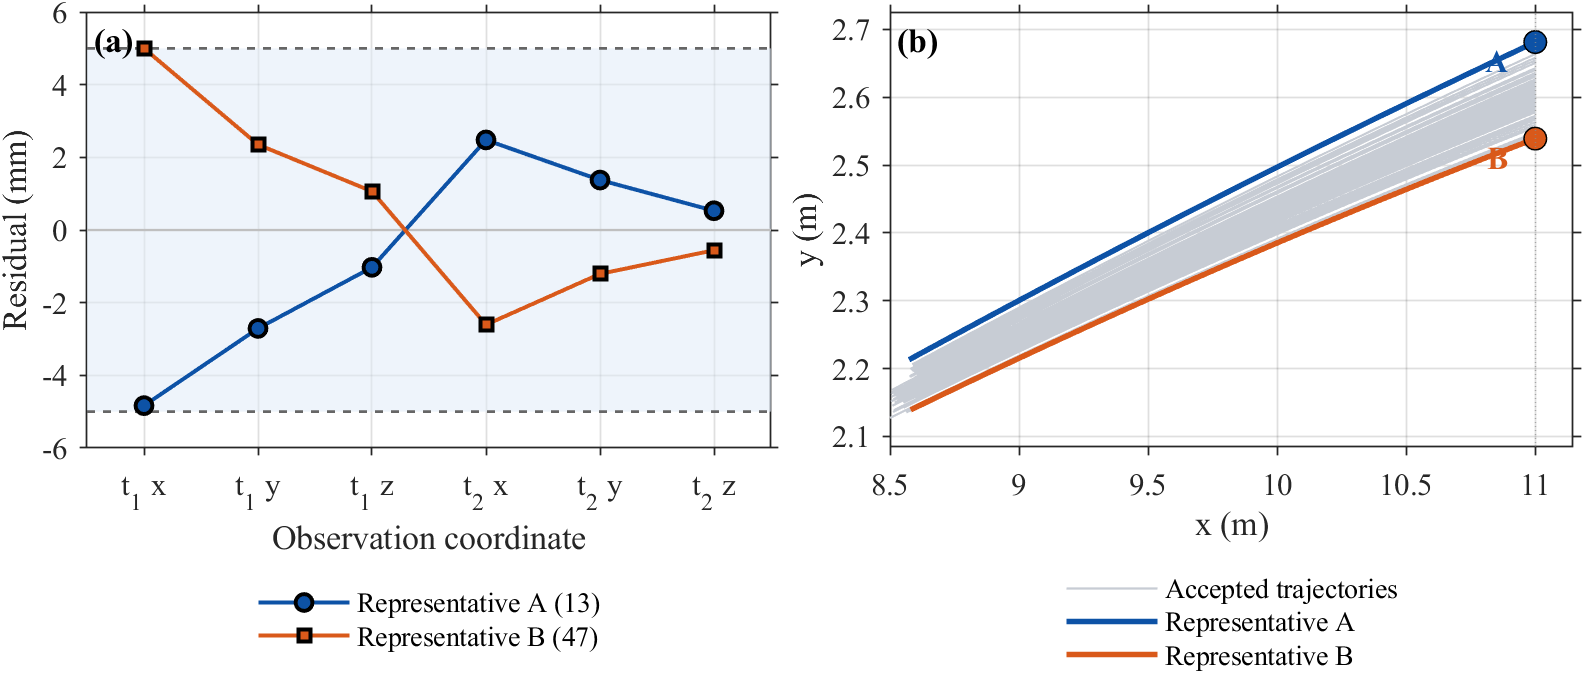
\includegraphics[width=.96\linewidth]{观测约束与轨迹分离.png}
\caption{两条符合观测的轨迹都通过六个坐标检查（左），但后程水平轨迹发生分离（右）。浅色带为声明的允许误差；位移按真实比例绘制。}
\label{fig:separation}
\end{figure}

图~\ref{fig:coupling}展示参数之间的联动。对这组观测，密度与阻力系数的乘积越大，通常需要更高的初速度（左）；横风变化时，计算出的侧向系数也会变化（中）；允许误差放宽后，能通过检查的参数组合随之增加（右）。
\begin{figure}[H]\centering
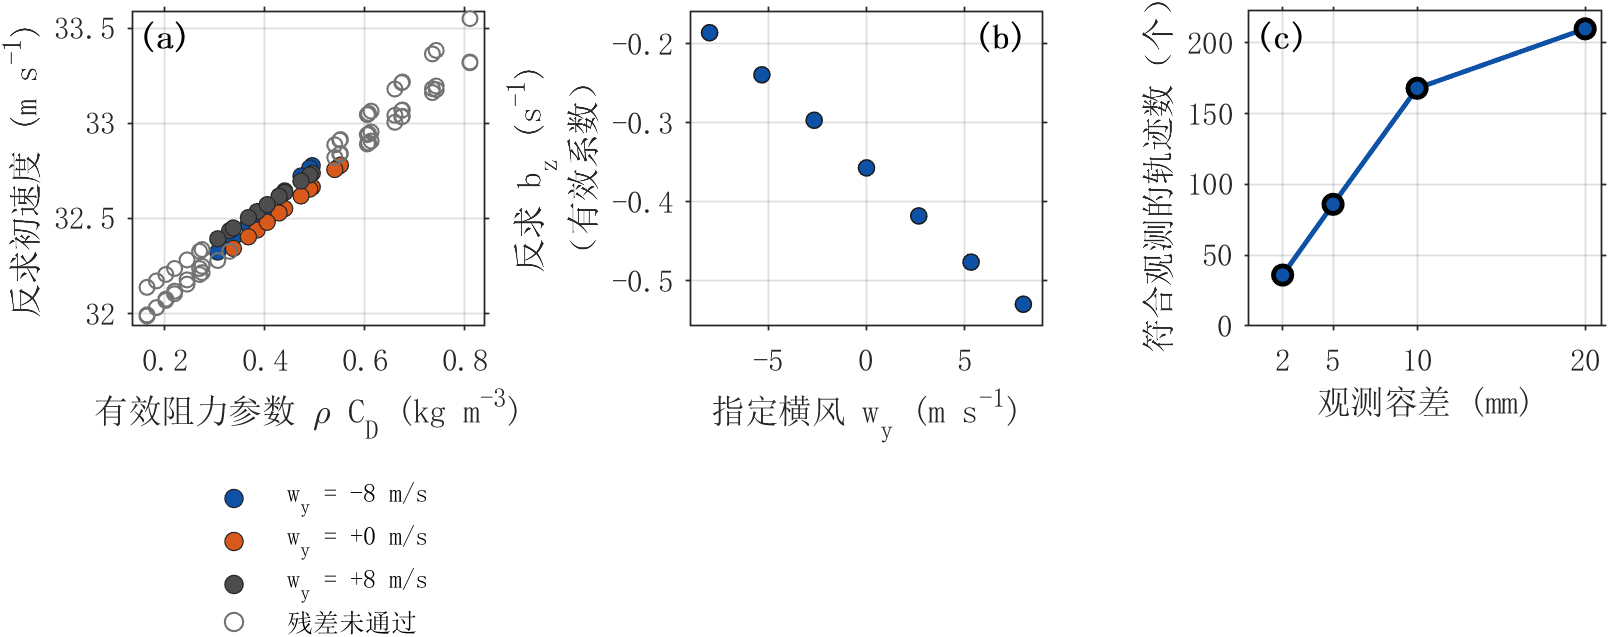
\includegraphics[width=\linewidth]{参数耦合与筛选敏感性.png}
\caption{参数耦合与筛选：三个风速切片中密度--阻力乘积与反求初速（左）；横风与被接受轨迹的反求 $b_z$（中）；允许误差与被接受数量（右）。所有数量都只针对列出的参数。}
\label{fig:coupling}
\end{figure}

图~\ref{fig:scatter}直接展示符合观测的轨迹在球门平面上的落点范围。颜色表示指定的阻力系数。点的密集程度由采样取值决定，不能据此判断哪一个落点更可能发生。
\begin{figure}[H]\centering
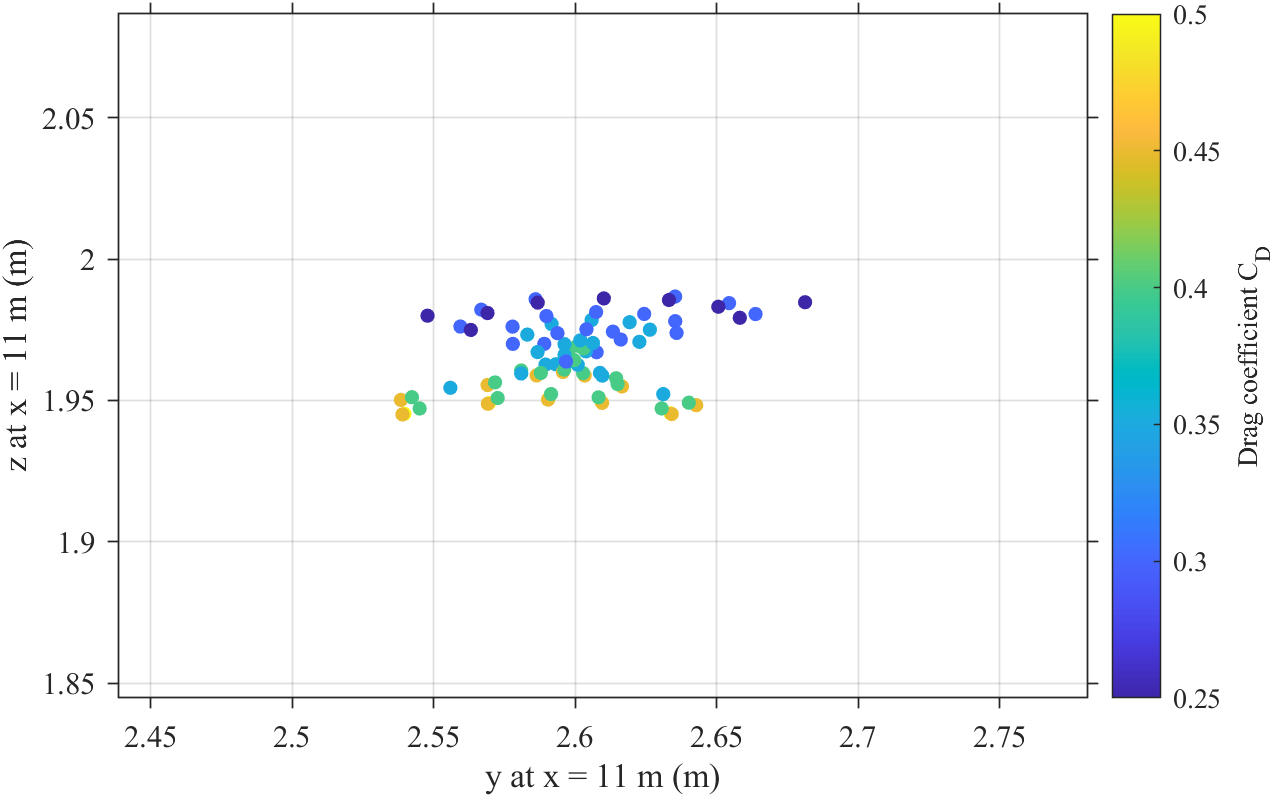
\includegraphics[width=.72\linewidth]{全程约束球门散点.png}
\caption{被接受轨迹在球门平面的落点。颜色表示列出的阻力系数。分散来自采样的参数取值，不是概率分布。}
\label{fig:scatter}
\end{figure}

另有一个交互界面允许横风 $[-15,15]$ m/s、密度 $[0.90,1.40]$ kg/m$^3$、$C_D\in[0.08,0.80]$；这只是范围更大的探索，与论文网格不同，筛选规则相同。

\section{计算检查与适用范围}
本节列出 MATLAB 内部做过的检查，以及这个结果的适用边界。

所有计算使用同一套方程和事件定义。三档步长只改变积分的最大步长，因此检验的是数值敏感性，而不是另一个模型。根据式~\eqref{eq:energy}推导的功与能关系，检查累积残差：
\begin{equation}
R_E(t)=E(t)-E(0)-\int_0^t(\mathbf F_D+\mathbf F_M)\cdot\mathbf v\,d\tau.
\end{equation}
事件检查确认触地、向前穿过 $x=11$ m 以及超时都被分别定位并记录。三档步长下球门平面落点的最大变化为 $6.66\times 10^{-15}$ m。该功与能累积残差的最大值为 $1.99\times 10^{-13}$ J。人为设置的过大初速度和侧向力均被检查程序拒绝。

这些检查检验的是程序与内部的能量平衡。没有独立的实测全程飞行，因此它们不能证明这只球、这块场地和这台相机服从该模型。报出的落点和范围只对列出的参数取值和声明的允许误差成立，不带概率，也不能保证搜索范围之外的情况。放宽允许误差会接受更多轨迹，但不会把采样得到的分散范围变成置信区间。

\clearpage
\section{结论}
本节回答问题。

仅有早期两个位置，在风和空气动力系数未知时，无法恢复唯一轨迹。对每一组列出的环境取值，仍可反求能重现两个位置的出脚条件；这些被接受的轨迹在球门平面上的落点并不相同。当前示例取风速 8.0 m/s、密度 1.225 kg/m$^3$ 时，球心在 0.4042 s 后穿过球门平面于 $(2.6087,1.9598)$ m。在列出的参数中，210 组里有 86 组通过 5 mm 检查，落点覆盖 $y\in[2.5384,2.6812]$ m、$z\in[1.9451,1.9867]$ m，其中两条符合观测的轨迹相距 0.1477 m。这些范围只描述采样网格，不是概率。更多观测时刻、实测风速和实测阻力系数可以缩小答案。

\begingroup\small\raggedright
\begin{thebibliography}{9}
\bibitem{upc} University Physics Competition. 2026 contest, Problem B. \url{https://www.uphysicsc.com/2026contest.html}. 访问于 2026 年 11 月 7 日.
\bibitem{ifab} The IFAB. Laws of the Game, Law 2: The Ball. \url{https://www.theifab.com/laws/latest/the-ball/}. 访问于 2026 年 11 月 7 日.
\bibitem{asai} T. Asai, K. Seo, O. Kobayashi and R. Sakashita. Fundamental aerodynamics of the soccer ball. \emph{Sports Engineering} 10, 101--109 (2007). \url{https://doi.org/10.1007/BF02844207}.
\bibitem{nasa} NASA Glenn Research Center. Drag Equation. \url{https://www1.grc.nasa.gov/beginners-guide-to-aeronautics/drag-equation/}.
\bibitem{ode} MathWorks. \texttt{ode45}: Solve nonstiff differential equations. \url{https://www.mathworks.com/help/matlab/ref/ode45.html}. 使用 MATLAB R2024a 实现.
\bibitem{lsq} MathWorks. \texttt{lsqnonlin}: Solve nonlinear least-squares problems. \url{https://www.mathworks.com/help/optim/ug/lsqnonlin.html}.
\end{thebibliography}

\smallskip\small
\section*{人工智能使用报告}
人工智能工具协助了代码生成、数值检查和文稿起草。所有采用的内容须由队员核验并负责。

\textbf{队号和完整 AI 记录待补，尚非提交终稿。}竞赛规则要求附上所用 AI 工具的完整输入与输出，该记录须在提交前补全并复核。
\endgroup
\end{document}
